\begin{figure}[H]
	\centering
	

	
	%\begin{subfigure}[b]{0.4\textwidth}
	%	\centering
	%	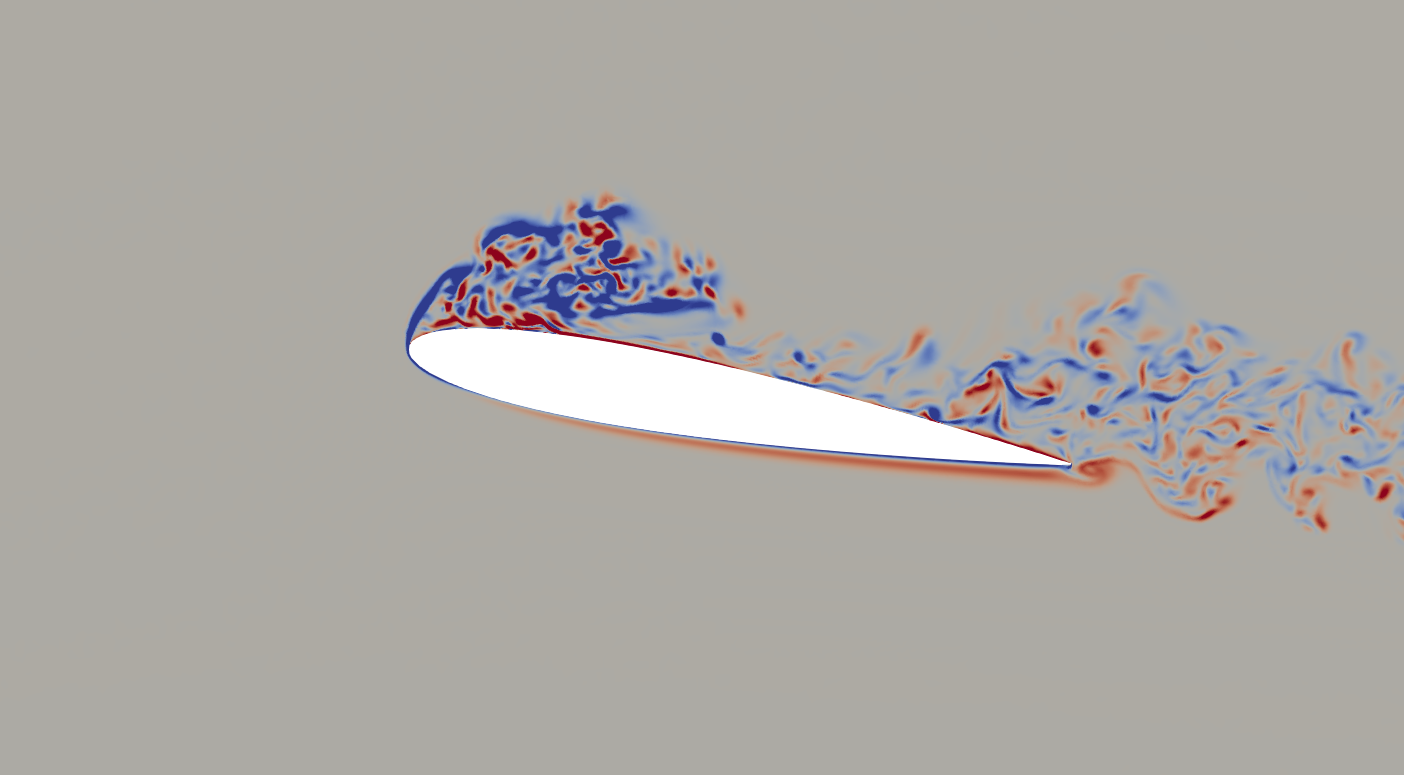
\includegraphics[width=1\textwidth]{figures/zonal_adapt_results/AC/mu_1pt5/baseline/phase_210.png}
	%	\caption{ $\psi$ = $210^\circ$, $\tilde{t}=0.583$}
	%	\label{fig:mu_1pt5_baseline_psi210}
	%\end{subfigure}
	%\begin{subfigure}[b]{0.4\textwidth}
	%	\centering
	%	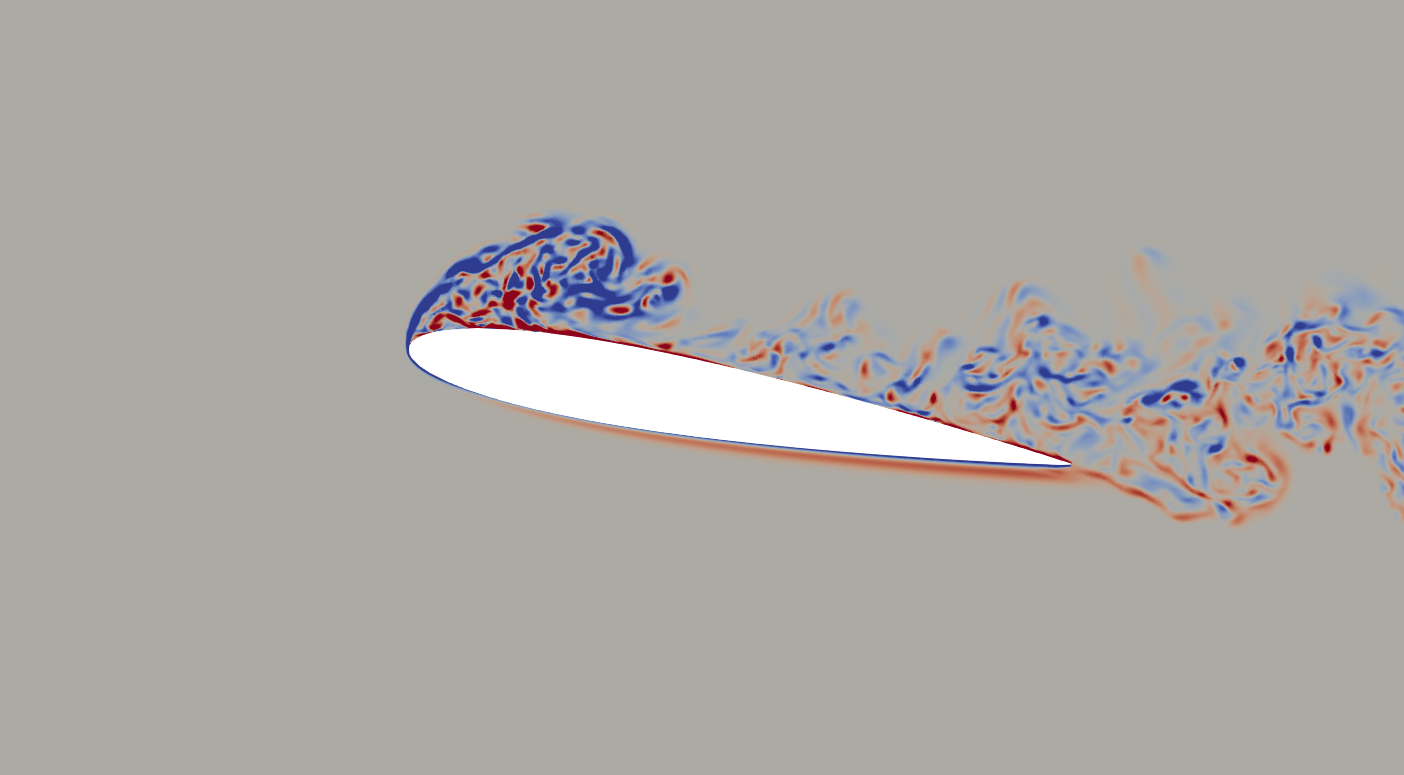
\includegraphics[width=1\textwidth]{figures/zonal_adapt_results/AC/mu_1pt5/AC/phase_210.png}
	%	\caption{ $\psi$ = $210^\circ$, $\tilde{t}=0.583$}
	%	\label{fig:mu_1pt5_AC_psi210}
	%\end{subfigure}	
	
	
	\begin{subfigure}[b]{0.4\textwidth}
		\centering
		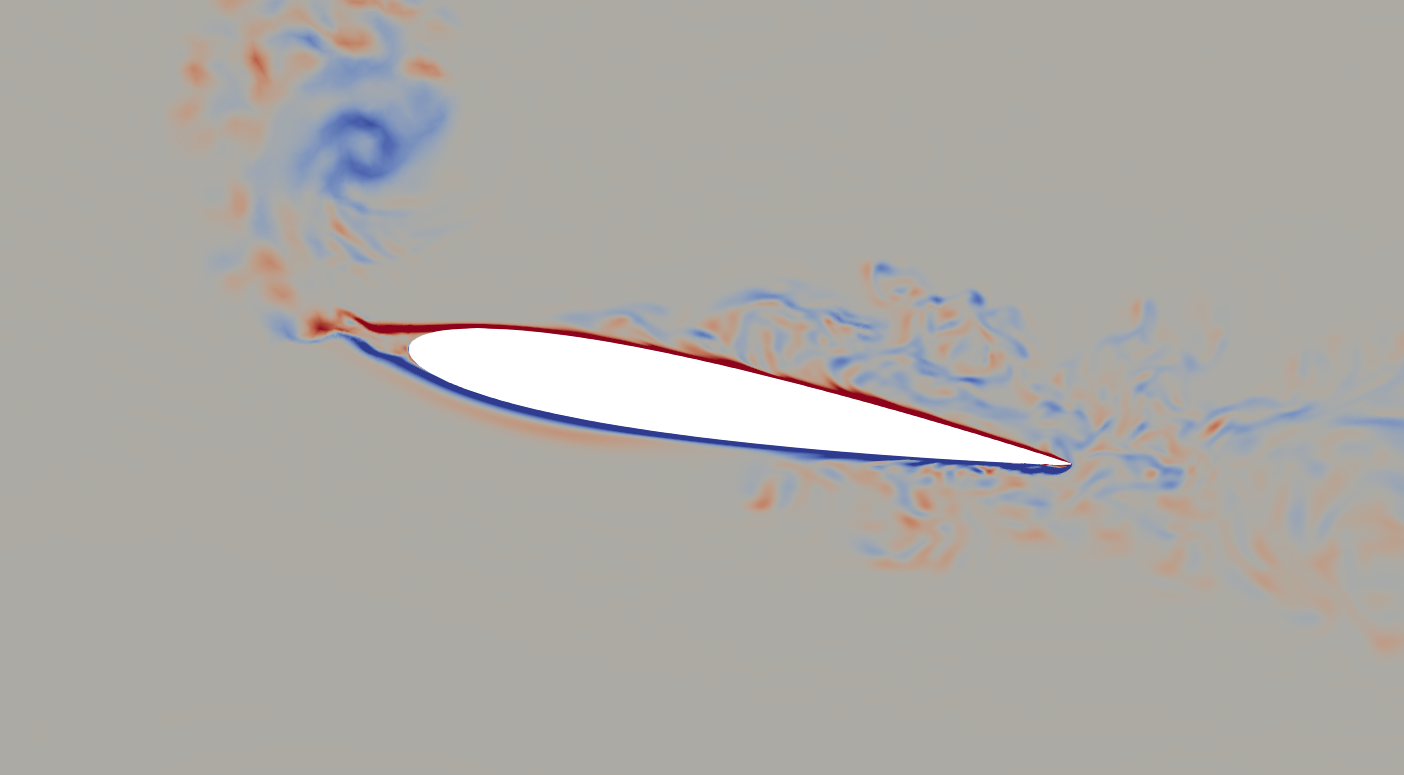
\includegraphics[width=1\textwidth]{figures/zonal_adapt_results/AC/mu_1pt5/baseline/phase_240.png}
		\caption{ $\psi$ = $240^\circ$, $\tilde{t}=0.667$}
		\label{fig:mu_1pt5_baseline_psi240}
	\end{subfigure}
	\begin{subfigure}[b]{0.4\textwidth}
		\centering
		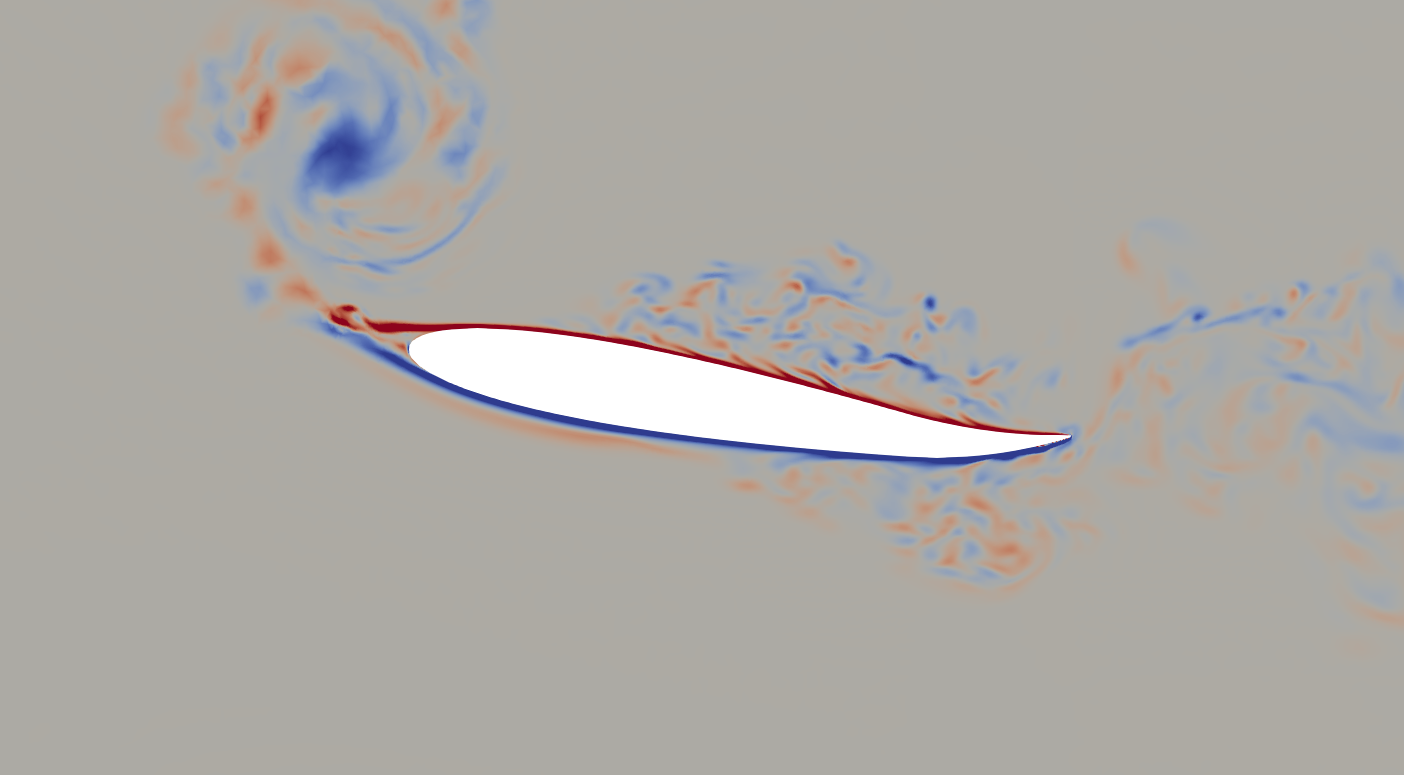
\includegraphics[width=1\textwidth]{figures/zonal_adapt_results/AC/mu_1pt5/AC/phase_240.png}
		\caption{ $\psi$ = $240^\circ$, $\tilde{t}=0.667$}
		\label{fig:mu_1pt5_AC_psi240}
	\end{subfigure}
	
	\begin{subfigure}[b]{0.4\textwidth}
		\centering
		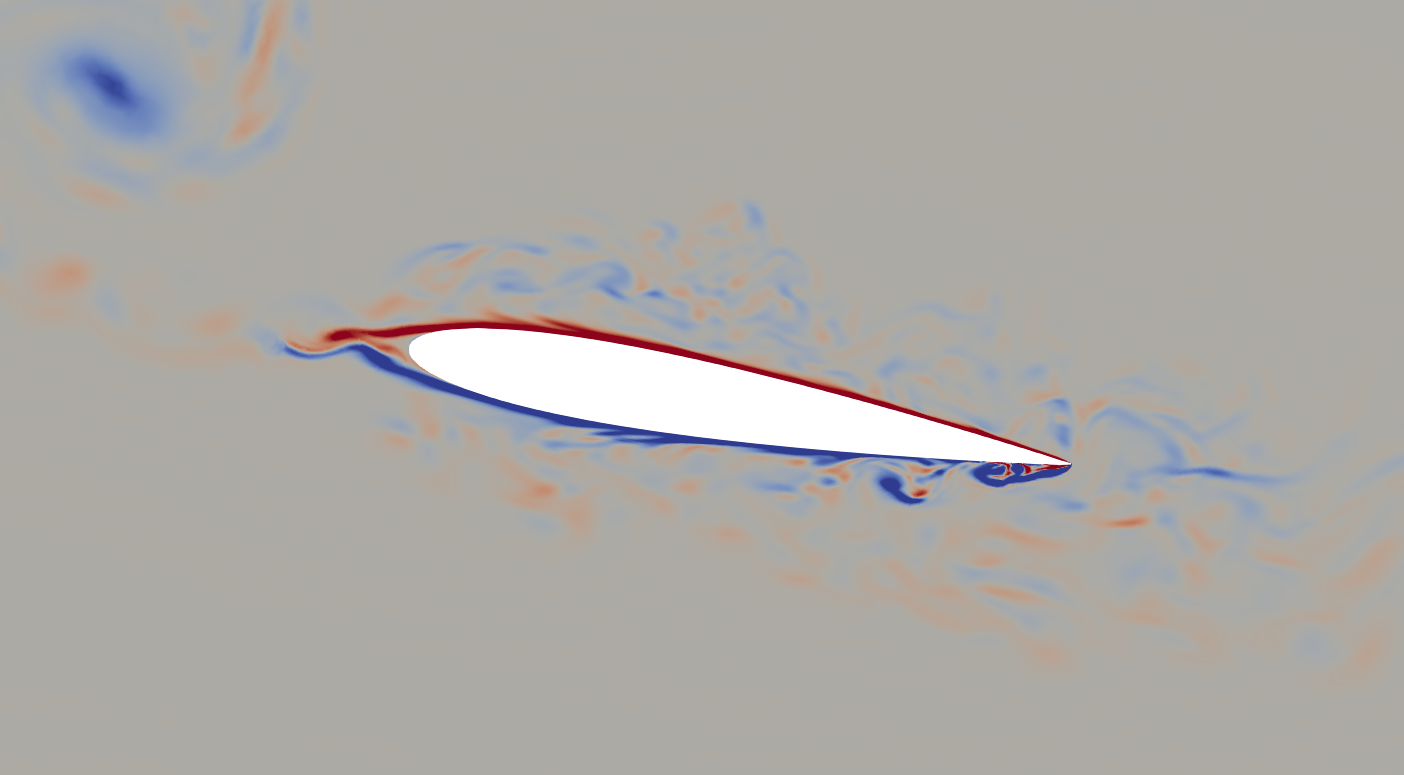
\includegraphics[width=1\textwidth]{figures/zonal_adapt_results/AC/mu_1pt5/baseline/phase_255.png}
		\caption{ $\psi$ = $255^\circ$, $\tilde{t}=0.708$}
		\label{fig:mu_1pt5_baseline_psi255}
	\end{subfigure}
	\begin{subfigure}[b]{0.4\textwidth}
		\centering
		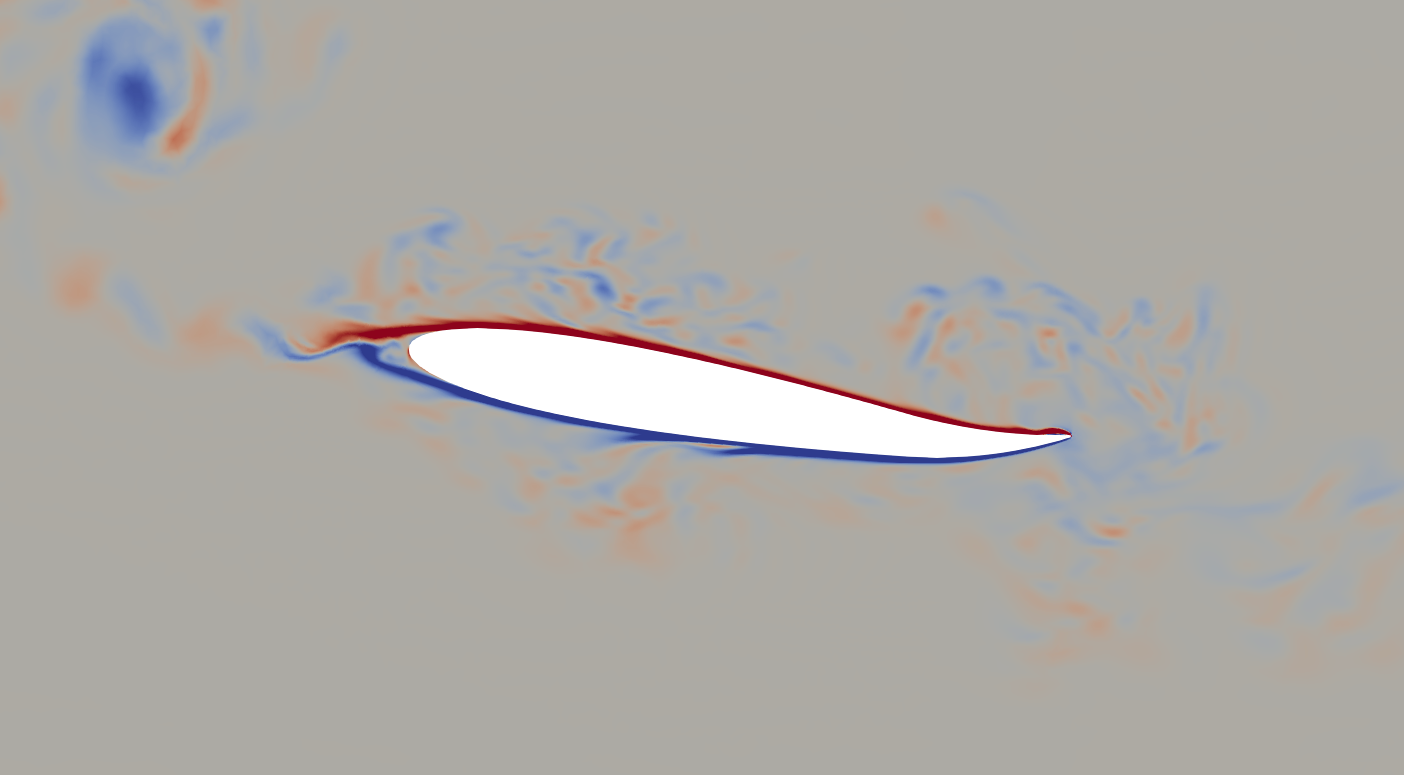
\includegraphics[width=1\textwidth]{figures/zonal_adapt_results/AC/mu_1pt5/AC/phase_255.png}
		\caption{ $\psi$ = $255^\circ$, $\tilde{t}=0.708$}
		\label{fig:mu_1pt5_AC_psi255}
	\end{subfigure}
	
	
	\caption{Instantaneous spanwise vorticity at 8 different phases for the baseline (left column) and actuated (right column) cases at $\mu_{sect}$ = 1.5}
	%\label{fig:vortScreen_mu1pt5}
\end{figure}

\begin{figure}[H]\ContinuedFloat
	\centering
	
	\begin{subfigure}[b]{0.4\textwidth}
		\centering
		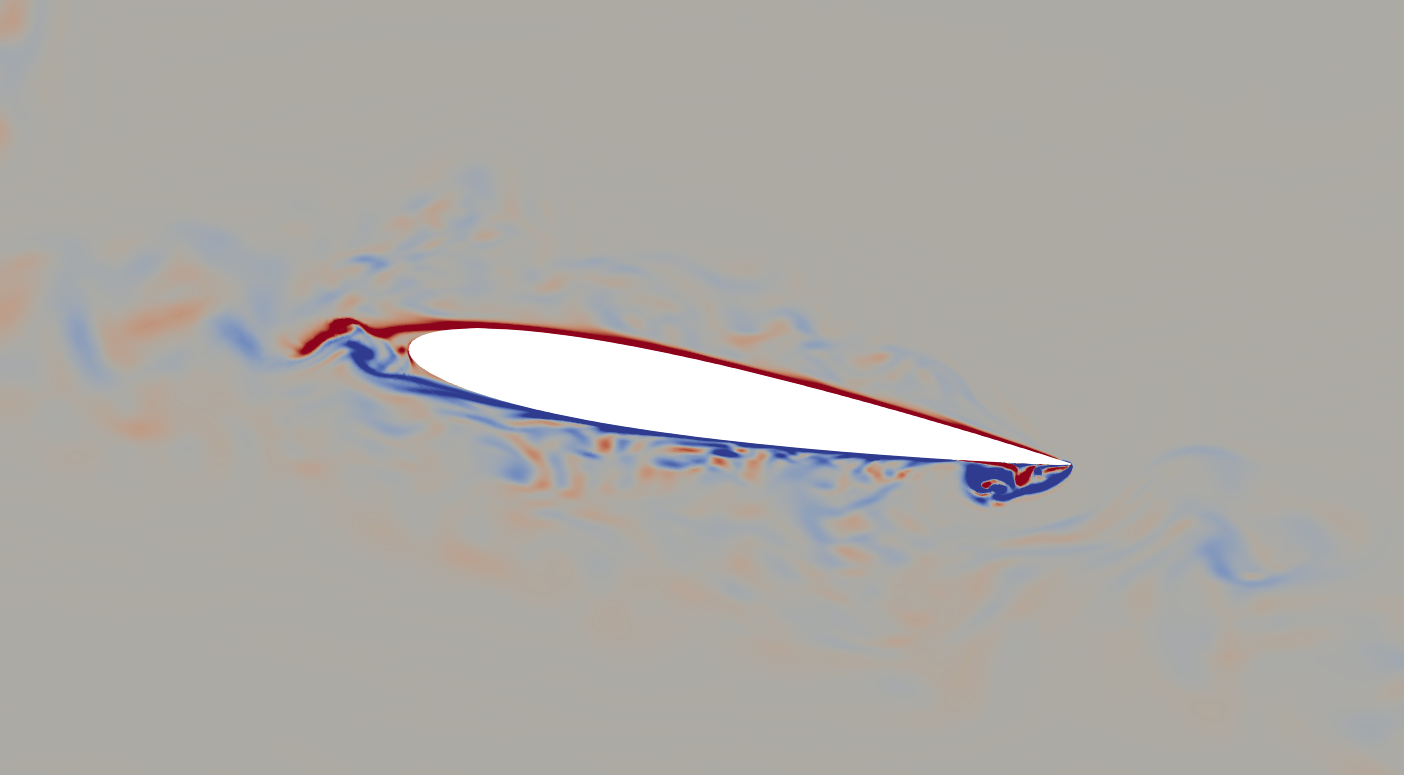
\includegraphics[width=1\textwidth]{figures/zonal_adapt_results/AC/mu_1pt5/baseline/phase_270.png}
		\caption{ $\psi$ = $270^\circ$, $\tilde{t}=0.75$}
		\label{fig:mu_1pt5_baseline_psi270}
	\end{subfigure}
	\begin{subfigure}[b]{0.4\textwidth}
		\centering
		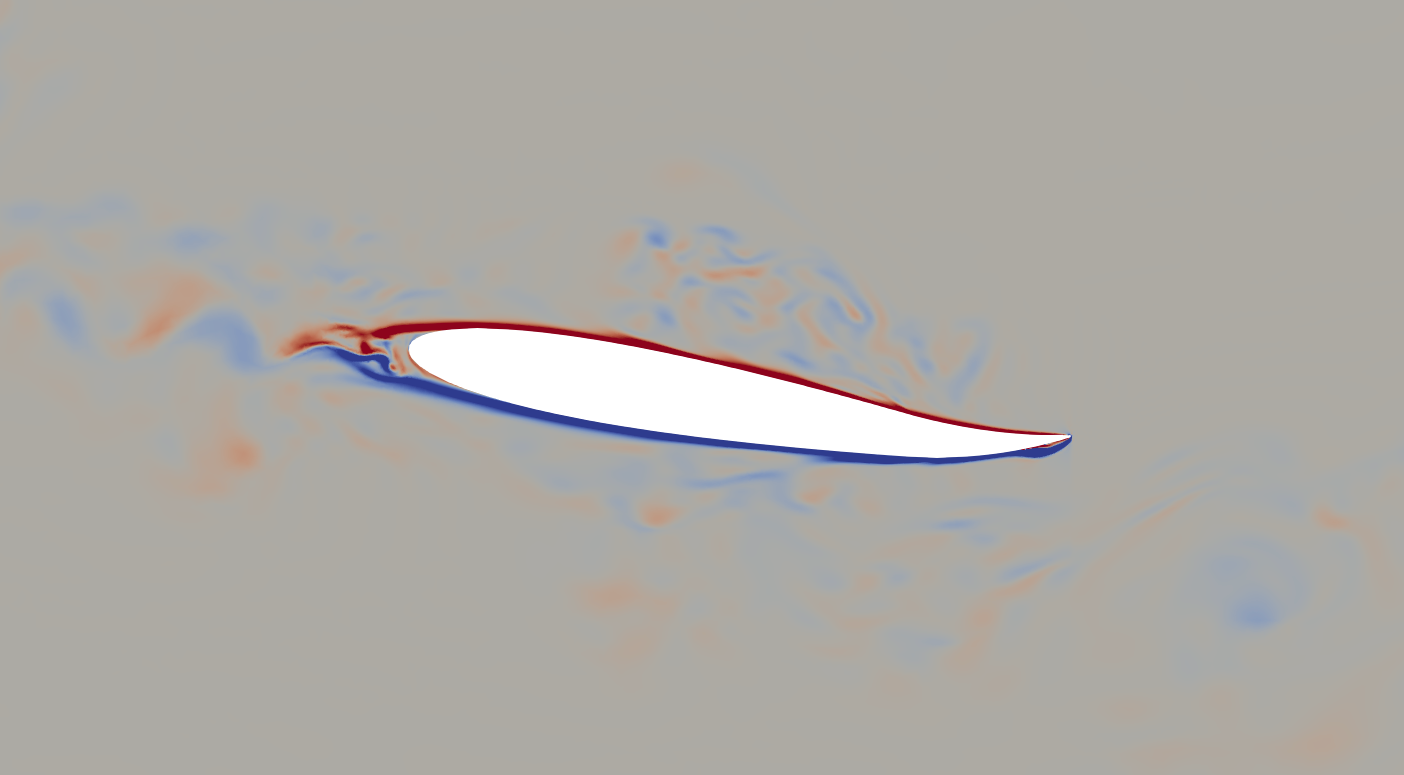
\includegraphics[width=1\textwidth]{figures/zonal_adapt_results/AC/mu_1pt5/AC/phase_270.png}
		\caption{ $\psi$ = $270^\circ$, $\tilde{t}=0.75$}
		\label{fig:mu_1pt5_AC_psi270}
	\end{subfigure}
	
	\begin{subfigure}[b]{0.4\textwidth}
		\centering
		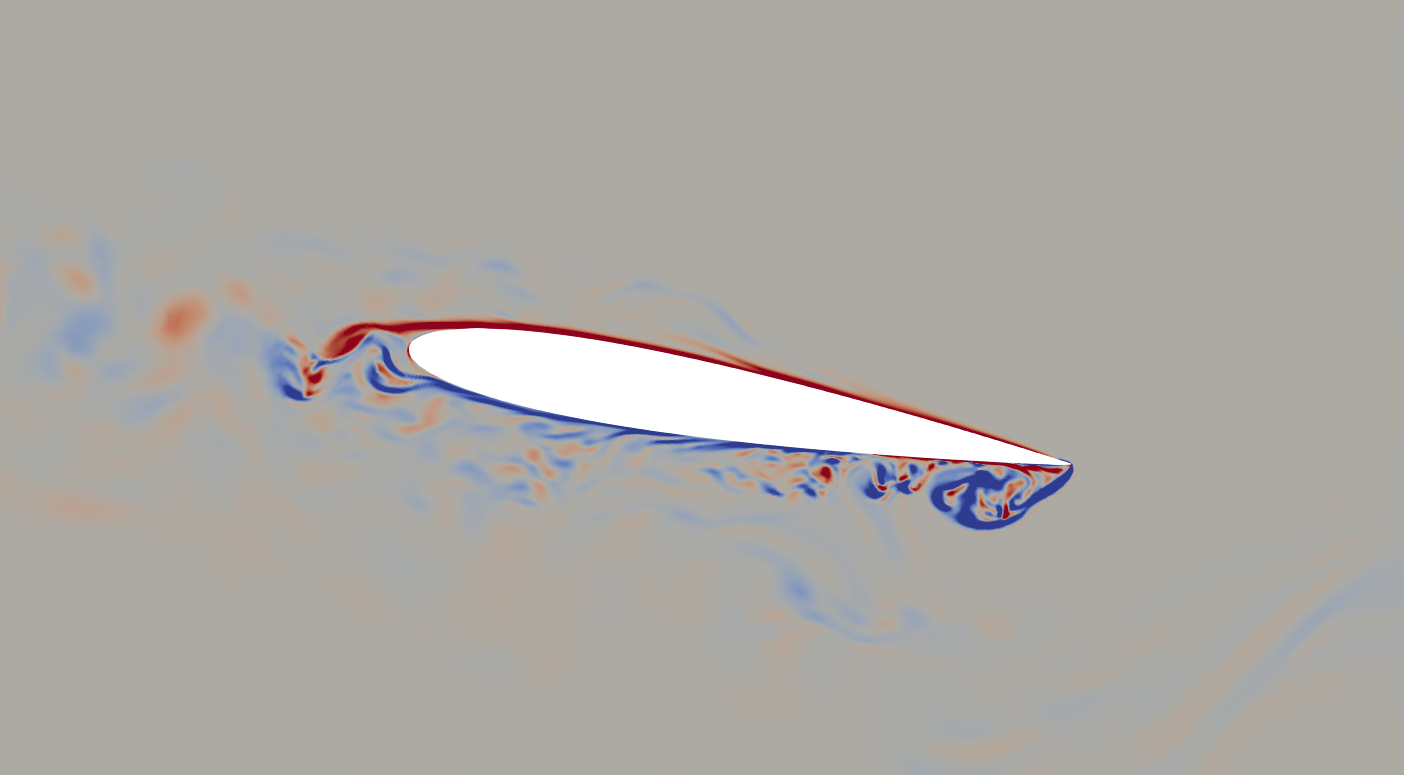
\includegraphics[width=1\textwidth]{figures/zonal_adapt_results/AC/mu_1pt5/baseline/phase_285.png}
		\caption{ $\psi$ = $285^\circ$, $\tilde{t}=0.792$}
		\label{fig:mu_1pt5_baseline_psi285}
	\end{subfigure}
	\begin{subfigure}[b]{0.4\textwidth}
		\centering
		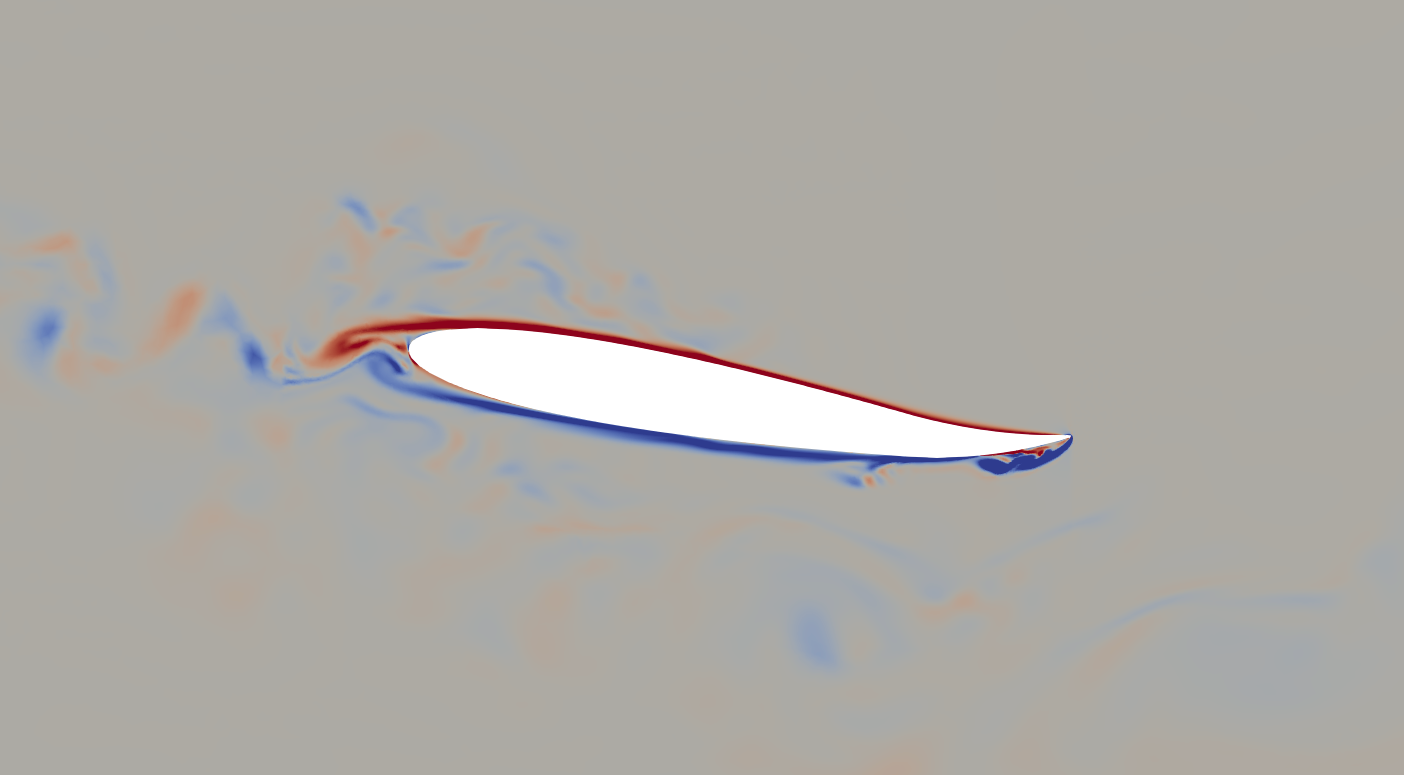
\includegraphics[width=1\textwidth]{figures/zonal_adapt_results/AC/mu_1pt5/AC/phase_285.png}
		\caption{ $\psi$ = $285^\circ$,  $\tilde{t}=0.792$}
		\label{fig:mu_1pt5_AC_psi285}
	\end{subfigure}
	
	
	%\begin{subfigure}[b]{0.4\textwidth}
	%	\centering
	%	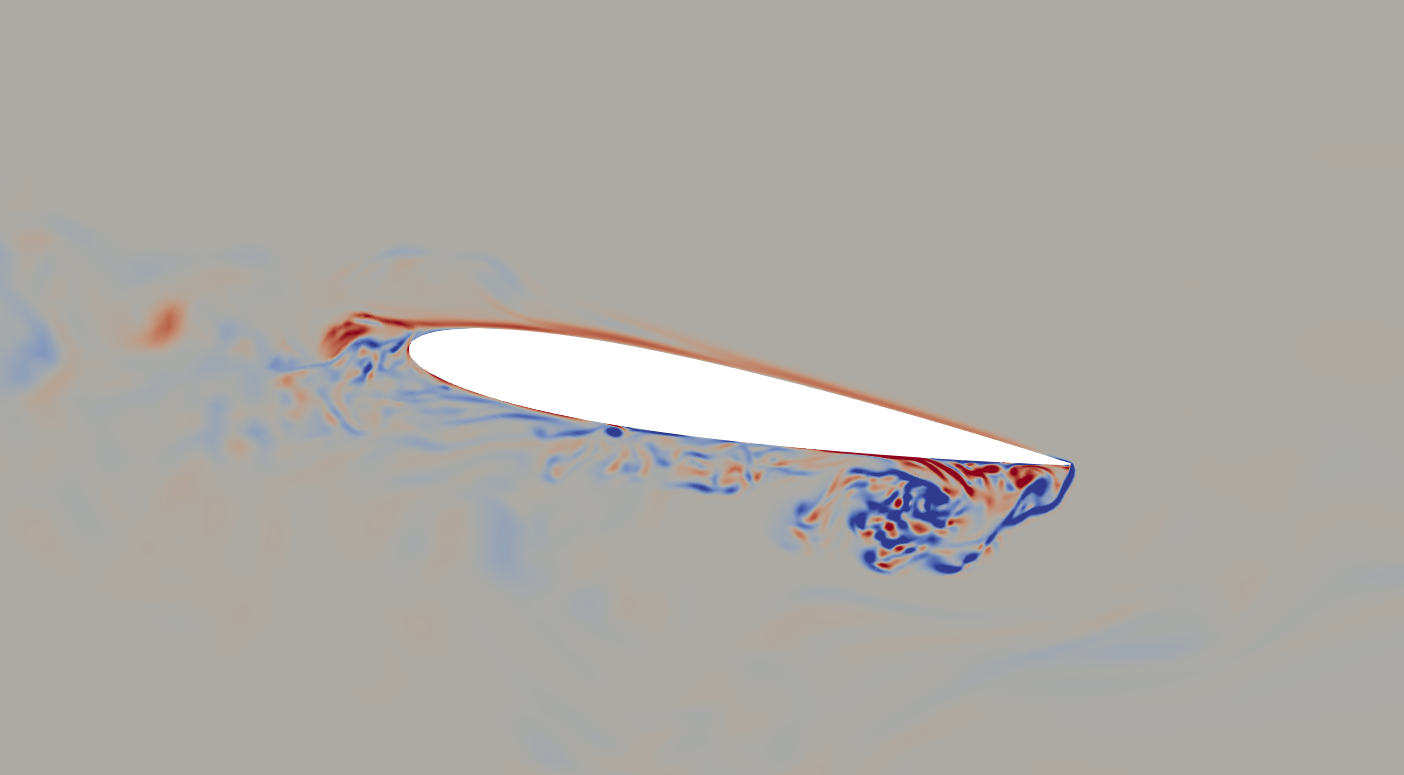
\includegraphics[width=1\textwidth]{figures/zonal_adapt_results/AC/mu_1pt5/baseline/phase_300.png}
	%	\caption{ $\psi$ = $300^\circ$, $\tilde{t}=0.833$}
	%	\label{fig:mu_1pt5_baseline_psi300}
	%\end{subfigure}
	%\begin{subfigure}[b]{0.4\textwidth}
	%	\centering
	%	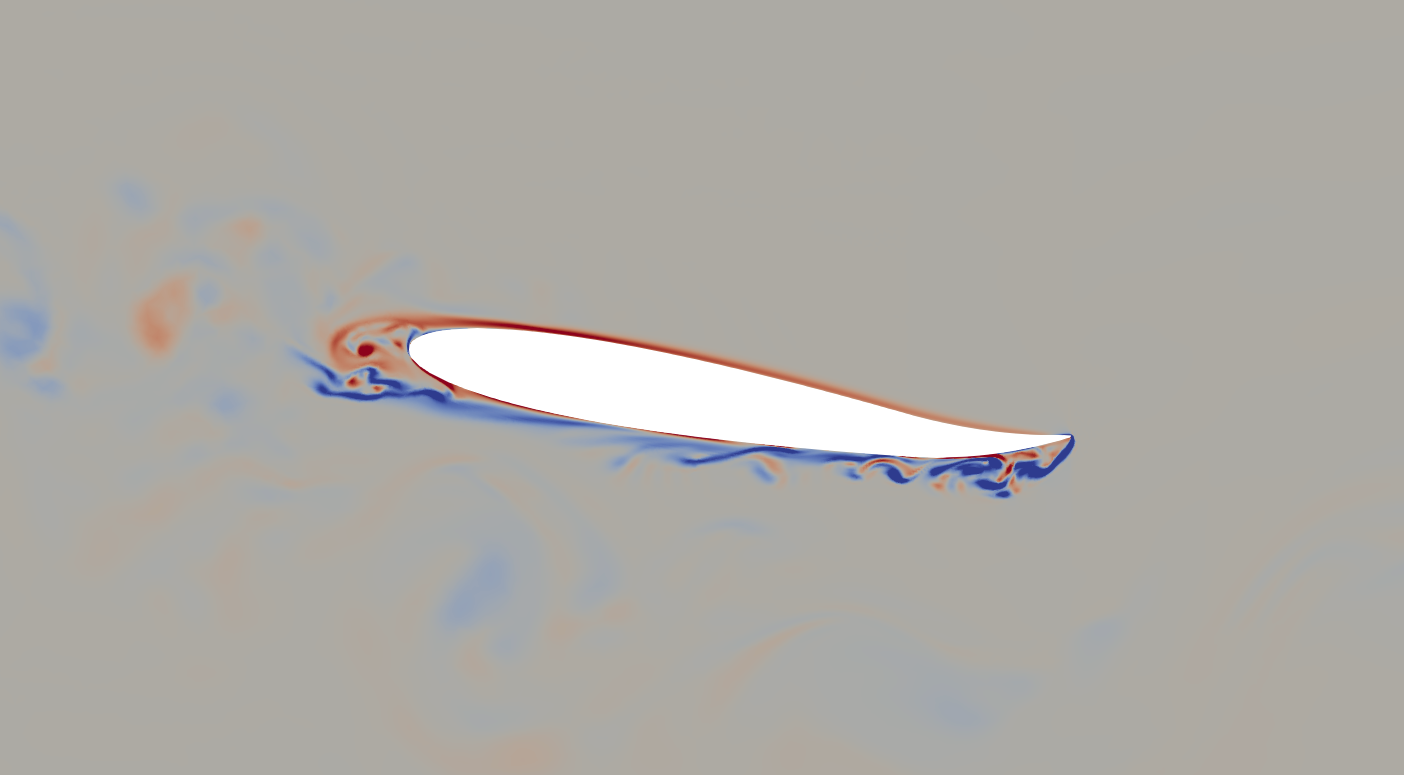
\includegraphics[width=1\textwidth]{figures/zonal_adapt_results/AC/mu_1pt5/AC/phase_300.png}
	%	\caption{ $\psi$ = $300^\circ$, $\tilde{t}=0.833$}
	%	\label{fig:mu_1pt5_AC_psi300}
	%\end{subfigure}
	
	\begin{subfigure}[b]{0.4\textwidth}
		\centering
		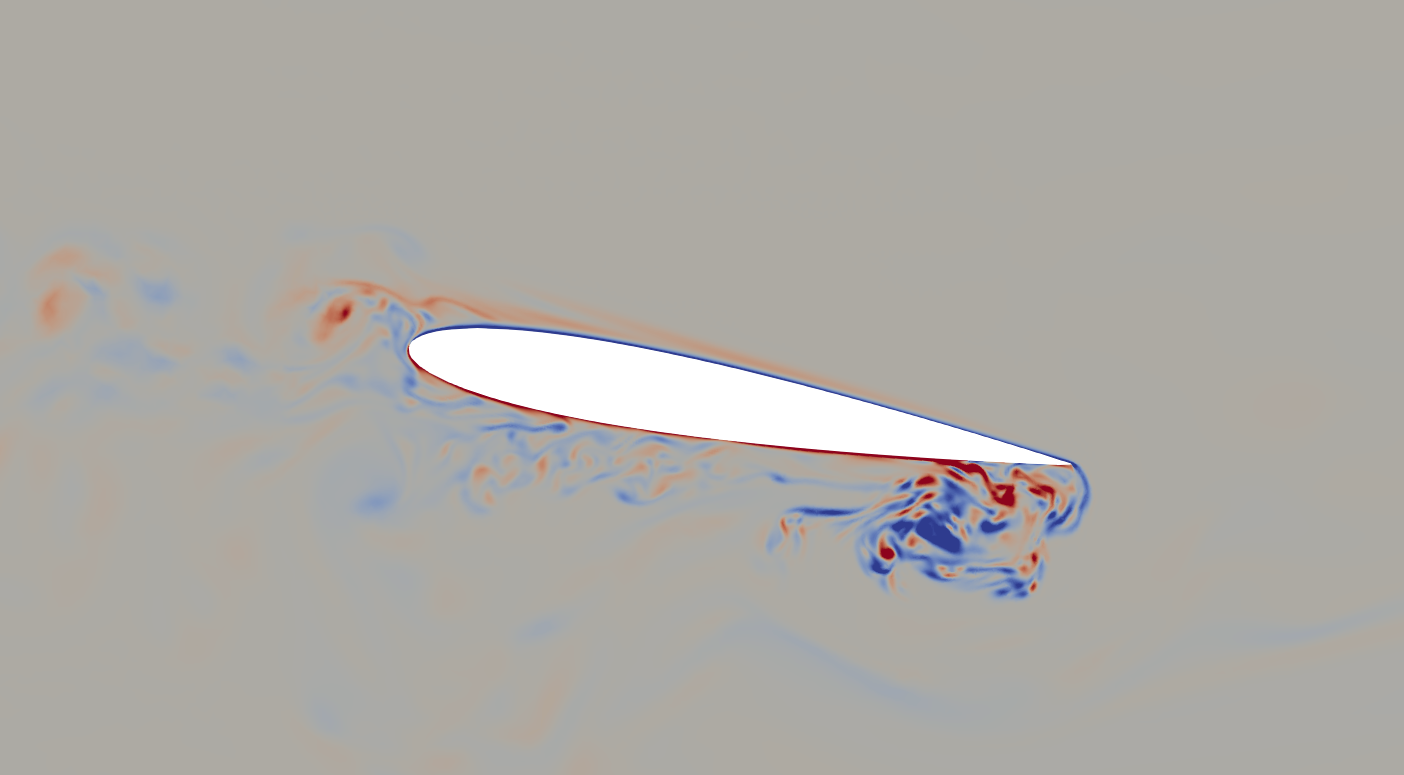
\includegraphics[width=1\textwidth]{figures/zonal_adapt_results/AC/mu_1pt5/baseline/phase_315.png}
		\caption{ $\psi$ = $315^\circ$, $\tilde{t}=0.875$}
		\label{fig:mu_1pt5_baseline_psi315}
	\end{subfigure}
	\begin{subfigure}[b]{0.4\textwidth}
		\centering
		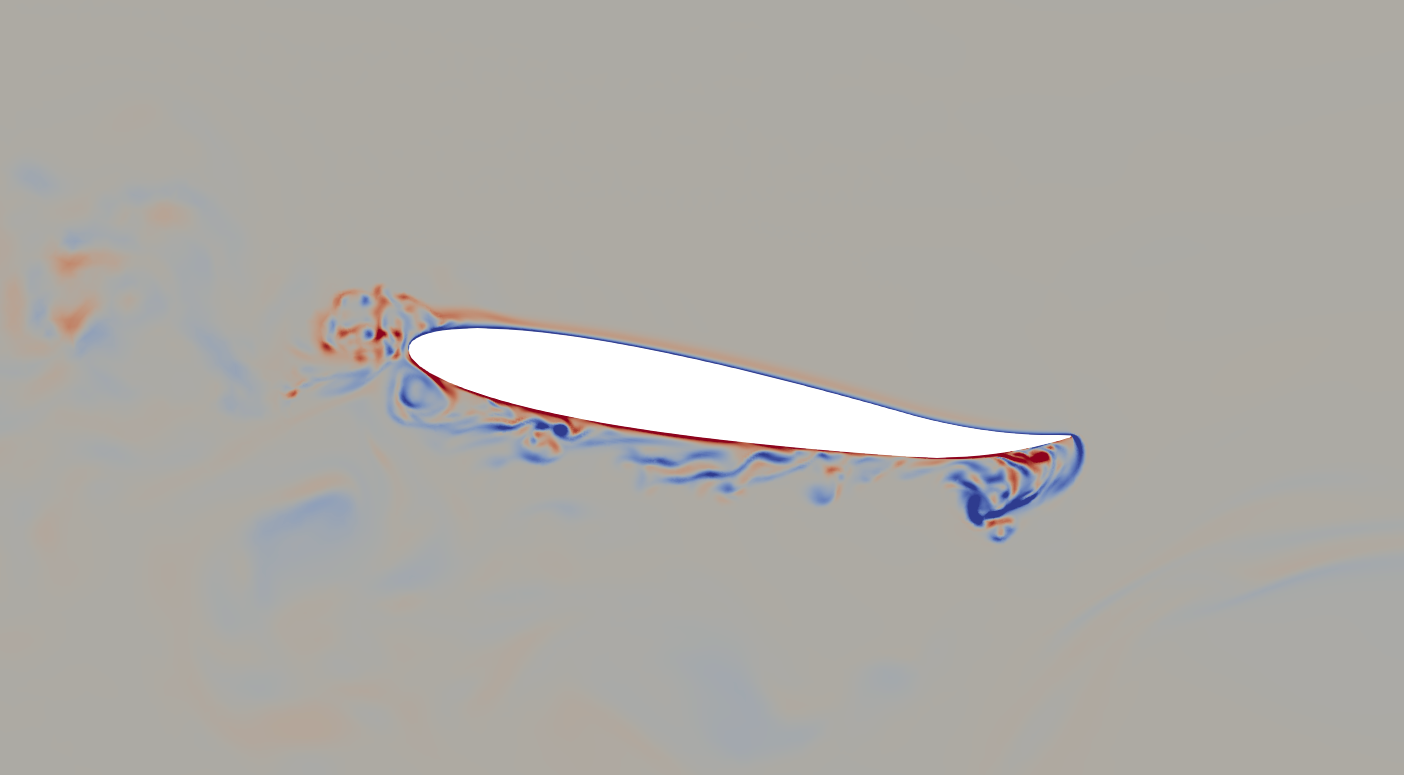
\includegraphics[width=1\textwidth]{figures/zonal_adapt_results/AC/mu_1pt5/AC/phase_315.png}
		\caption{ $\psi$ = $315^\circ$, $\tilde{t}=0.875$}
		\label{fig:mu_1pt5_AC_psi315}
	\end{subfigure}
	
	\begin{subfigure}[b]{0.4\textwidth}
		\centering
		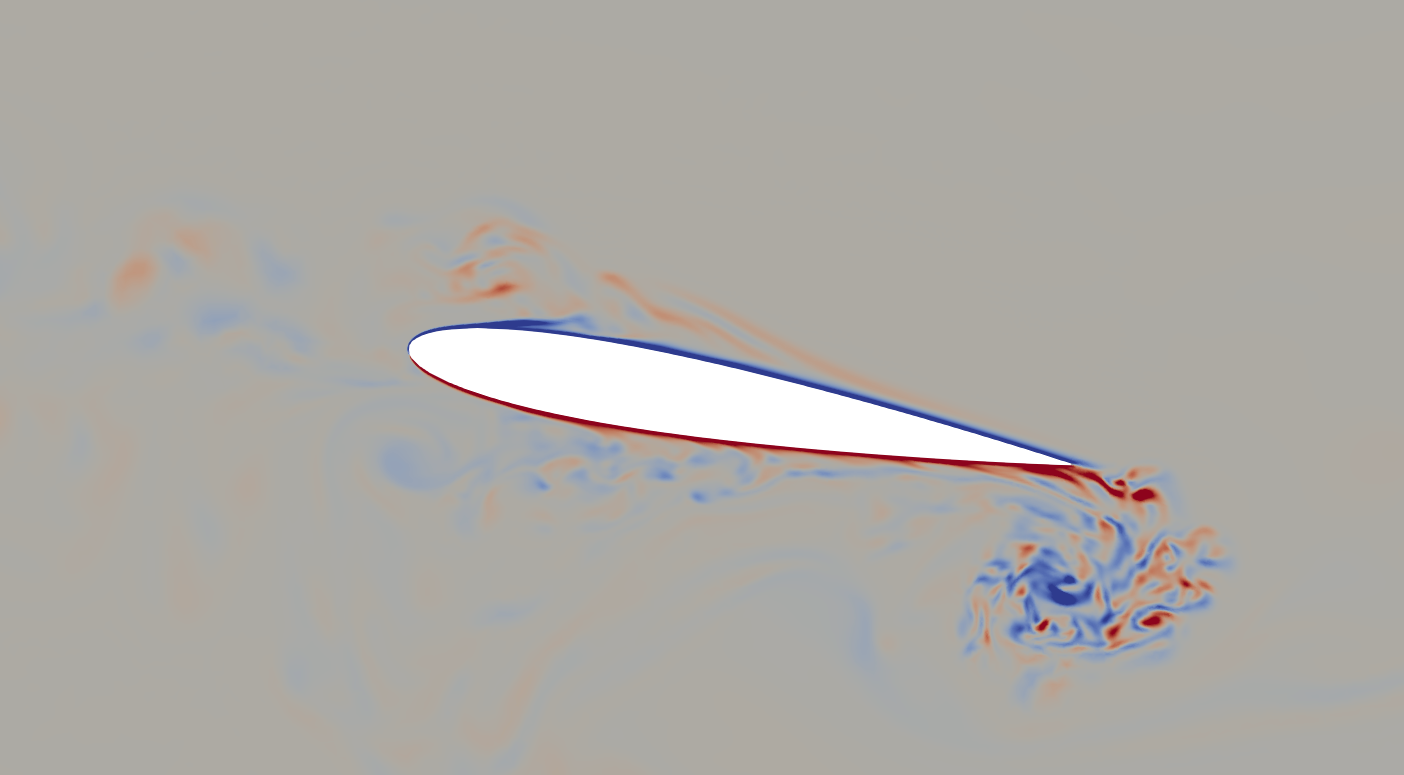
\includegraphics[width=1\textwidth]{figures/zonal_adapt_results/AC/mu_1pt5/baseline/phase_330.png}
		\caption{ $\psi$ = $330^\circ$, $\tilde{t}=0.917$}
		\label{fig:mu_1pt5_baseline_psi330}
	\end{subfigure}
	\begin{subfigure}[b]{0.4\textwidth}
		\centering
		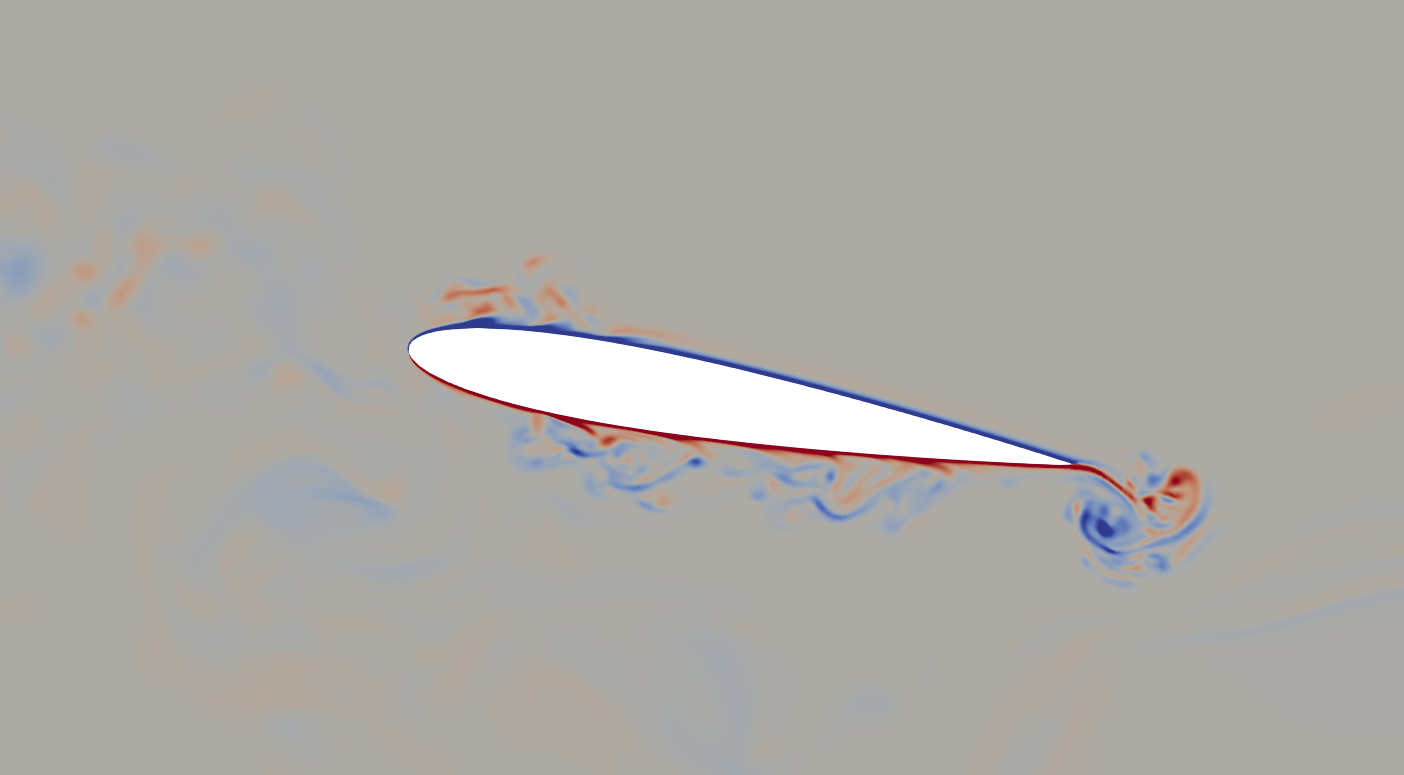
\includegraphics[width=1\textwidth]{figures/zonal_adapt_results/AC/mu_1pt5/AC/phase_330.png}
		\caption{ $\psi$ = $330^\circ$, $\tilde{t}=0.917$}
		\label{fig:mu_1pt5_AC_psi330}
	\end{subfigure}
	
	%\begin{subfigure}[b]{0.4\textwidth}
	%	\centering
	%	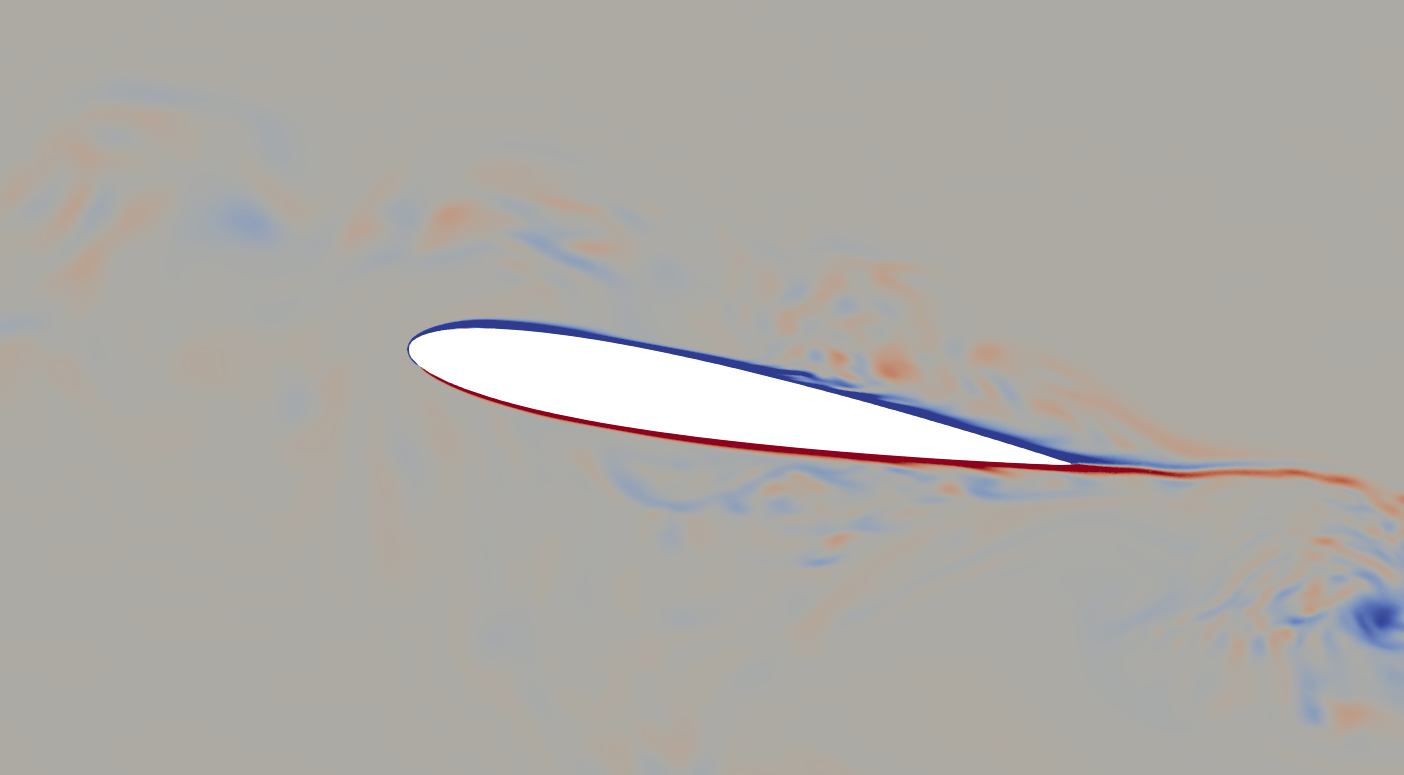
\includegraphics[width=1\textwidth]{figures/zonal_adapt_results/AC/mu_1pt5/baseline/phase_345.png}
	%	\caption{ $\psi$ = $345^\circ$, $\tilde{t}=0.958$}
	%	\label{fig:mu_1pt5_baseline_psi345}
	%\end{subfigure}
	%\begin{subfigure}[b]{0.4\textwidth}
	%	\centering
	%	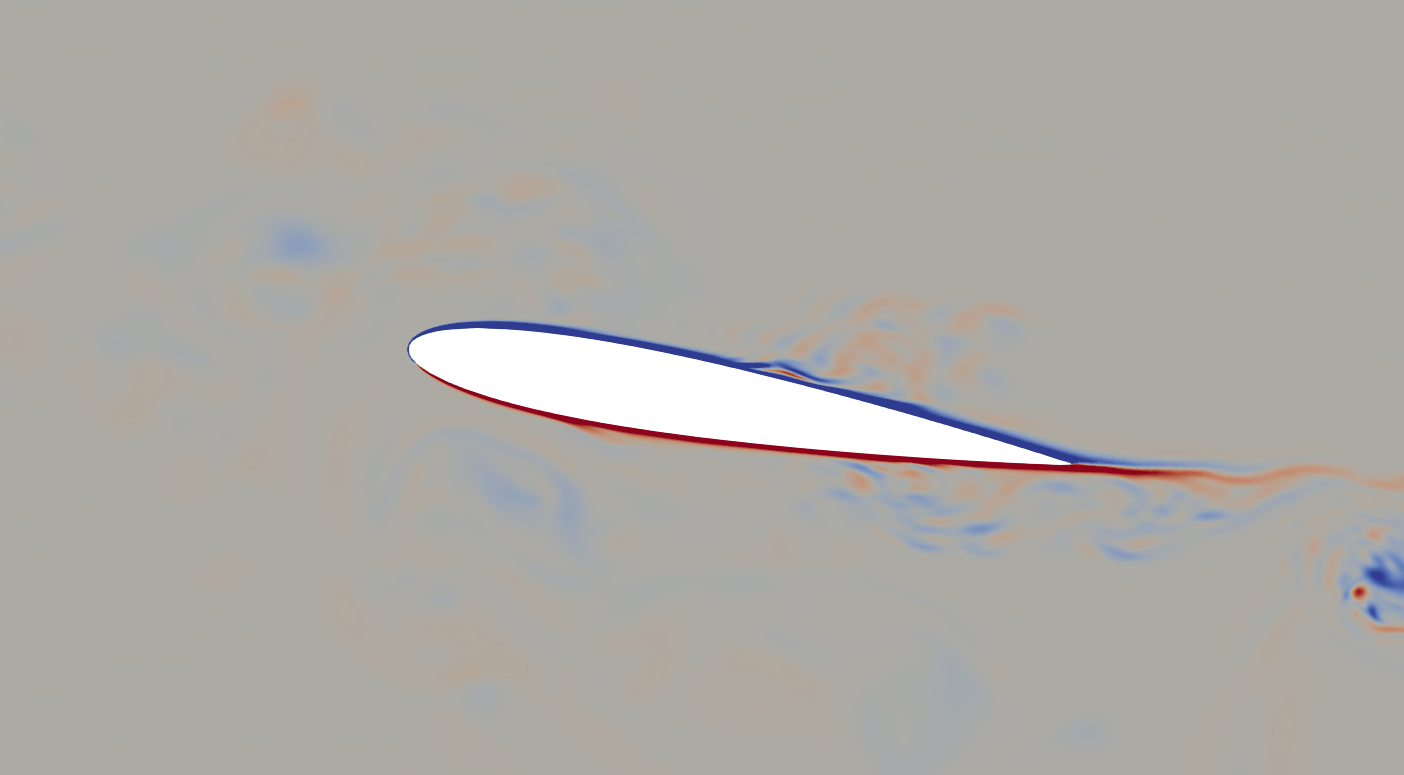
\includegraphics[width=1\textwidth]{figures/zonal_adapt_results/AC/mu_1pt5/AC/phase_345.png}
	%	\caption{ $\psi$ = $345^\circ$, $\tilde{t}=0.958$}
	%	\label{fig:mu_1pt5_AC_psi345}
	%\end{subfigure}
	
	
	
	\caption{Instantaneous spanwise vorticity at 8 different phases for the baseline (left column) and actuated (right column) cases at $\mu_{sect}$ = 1.5}
	\label{fig:vortScreen_mu1pt5}
\end{figure}
